\newpage
\chapter{Small Screens Optimisation}
\section{Design Ideas}

Bellow pictures represents the same content using a layout suitable for small devices in portrait and landscape orientation.

\begin{figure}[h!]
\begin{tabular}{ c c }
		\setlength\fboxsep{0pt}
		\setlength\fboxrule{1pt}
		\fbox{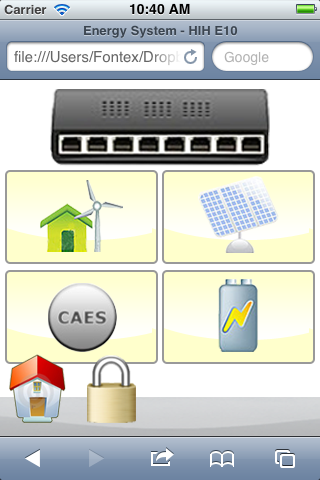
\includegraphics[width=0.4\textwidth]{images/portrait.png}}
&
		\setlength\fboxsep{0pt}
		\setlength\fboxrule{1pt}
		\fbox{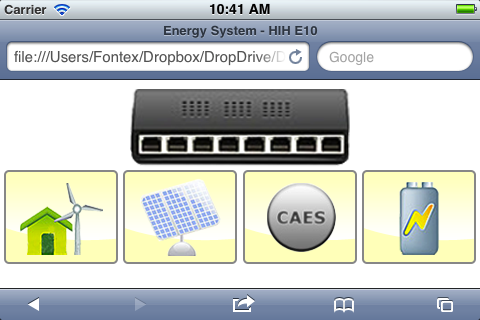
\includegraphics[width=0.55\textwidth]{images/landscape.png}}
\end{tabular}
\caption{Layout Proposal}
\end{figure} 

\section{Constrains and Limitations}
On small screens horizontal scroll bar is not an option, since it breaks all the dynamics of the user experience, the processor is slower, the memory is limited so loading large file sizes is not a plus.\\
\\
\noindent \textbf{For small screen some limitations should be considered and applied to the design:}\\
- One column layout only, this will avoid the horizontal scroll bar.\\
- HTML optimised using efficient tags and attributes.\\
- CSS optimised with efficient styles proprieties.\\
- Minimise the amount of decorative images, or if needed, use of pre loaders (scripts that only show the page when fully loaded) so the user experience is not affected.\\
- Write good alternative text (attribute 'alt')  for images, so in case the image is not needed an alternative text could be shown for example navigation icons.\\
- Avoid effects that need mouse or keyboard events.\\
- Avoid the use of Javascript on layout design since some mobile browsers may be set to block this scripts.

\section{Screen Sizes Proposal}
Smaller screens will always be the tablet computers or the ones that fits on pockets like smartphones.\\
Keeping this in mind the most used screen sizes are:\\
- 320x480 Screen Size ( eg. iPhone )\\ 	% Tested on: iPhone3G(OK),iPhone 4(OK)
- 480x800 Screen Size (eg. HTC Titan, HTC Desire)\\ %HTC desire(NOK)
- 1024x600 Screen Size ( eg. Samsung Galaxy )\\
- 1024x768 Screen Size ( eg. iPad)\\
\\
\noindent \textbf{List of the most popular smartphones and tablet computers}\\
- Samsung Galaxy Player 5.0 (released 2011)\\
- Samsung Galaxy S II (released 2011)\\
- Apple iPhone 4S (released 2011)\\
- Apple iPhone 4 (released 2010)\\
- HTC Titan (released 2011)\\
\newpage
\section{Best Practices}

Mobile standards are not yet fully developed, but an initiative by the W3C (http://www.w3.org/Mobile/) describes some best practices for small devices web development. As HTML and CSS a Mobile checker can be found and used to identify possible threats for small screen devices.

Some best practices for mobile web development have to be adapted when developing to the new smartphones and tablets computers, since they are detected as normal screens because of they higher pixel resolution and browsers such as Safari, Chrome, etc. The mobile W3C checker have to be used more as a guideline and not as a strict design method.
\\
\\ \textbf{Content Selection:} on small screens all the data have to be more objective since all the information cannot be shown at once.\\
\\ \textbf{Interaction method:} its important to determine the type of interaction that the device have with the user, because this will change the layout it self. In this proposal devices (and the most used now a days) the interaction would be touch based, all events are related with the user directly touching the screen with the finger or a pen, for this kind of interactions:\\
- Event elements should be widely spaced from each others for the user to be able to touch them directly\\
- Event elements have to be large enough to be early selected.\\
\\\textbf{Use of client side capability detection:} Javascript and CSS media queries are the client side solutions for developers. Javascript may be blocked by the user so CSS media queries should be the first option. Server side device detection would be a best practice since the file size would get smaller and less requests would be made, but is not always possible.\\
\\\textbf{Scrolling:} limit scrolling to one direction, this is archived, by re-designing the page for one column only and setting the width of the content for the device screen width.\\
\\\textbf{File Size:} unnecessary spaces and all the comments should be removed, this will decrease the file size to be loaded by the device making the website loading faster.\\
\\\textbf{Server Requests:} decrease the number of server requests, this can be done by avoiding putting image elements on the HTML file.
\\\\
Some more mobile web practices takes in consideration are seen at \textit{http://www.w3.org/2007/02/mwbp\_flip\_cards}, this flip cards illustrate all the process of designing and testing a web application/page on a small screen device.

\section{HTML}

For a long time tables were used to make the webpages layout, this was made by nesting HTML table tags to create for example multi column pages, separate headers, main and footers, etc..

As solution, HTML should be used to the intellectual content of the page, while CSS determine how to represent the content to the user. This method of design improves the time of development since theres no more nested tables the HTML tags become more understandable, so create and redesigned a webpage becomes more easy and less time consuming, improves search engines rankings and files sizes diminished noticeable.
\newpage
\subsection{Head}

A small screen device should have less HTML elements tags, since not all the mobile browsers support all the tags, using W3C mobile as guide line, the use of the doctype mobile 1.2 is advised since this will keep the web page suitable for all kind of small screen devices and browsers.

\begin{lstlisting}
	<!DOCTYPE html PUBLIC "-//WAPFORUM//DTD XHTML Mobile 1.2//EN" "http://www.openmobilealliance.org/tech/DTD/xhtml-mobile12.dtd">
\end{lstlisting}


Meta tags in HTML is the information data, usually specifies a page description (viewport), keywords (words used by search engine bots to identify web pages contents), etc. This meta tags are defined in the head	element of the HTML file. 

\begin{lstlisting}
	<meta http-equiv="Content-Type" content="application/xhtml+xml; charset=UTF-8"/>
	<meta http-equiv="Cache-Control" content="max-age=3600, must-revalidate " />
	<meta name="viewport" content="width=device-width; maximum-scale=1.0; user-scalable=0;"/>
\end{lstlisting}

Cache is add to the HTML meta tags, this will help the device to load the web page faster and doing less requests to the server, this is a plus when the content of the web page is static. This method of setting HTML headers for cache is not the most reliable since some browsers might not read this meta tags, for a reliable caching-control a server-side HTTP headers script should be implemented.

HTML only contains the intellectual value of the web page, and no layout setting, so the layout setting are defined in CSS ( Cascade Style Sheet ), this are linked to the HTML page trough the tag \textit{<link>}.  Link tags defines the relationship between the HTML file and an external file, the mostly used and supported in all browsers are CSS documents.

\begin{lstlisting}
	<link rel="stylesheet" type="text/css" media="only screen and (orientation:portrait)" href="index_portrait.css" />
	<link rel="stylesheet" type="text/css" media="only screen and (orientation:landscape)" href="index_landscape.css" />
\end{lstlisting}

\begin{table}[h!]
\begin{tabular}{ | c | l | }
\hline
\textbf{Atribute} & \textbf{Description} \\ \hline
href & Location of the linked document. \\ \hline
del & Relationship between the current document and the linked document. \\ \hline
type & Specify the type of the linked document. \\ \hline
media & Defines which media should load the linked document. \\ \hline
\end{tabular}
\caption{Link tag atributes description.}
\end{table}
\newpage
\subsection{Re-Design}

A Javascript script will redirect a user accessing the index page through a small screen device to the small screens capable web site. This is the same as for desktops computers but smaller in graphics and HTML tags since some devices can only put in cache 25KB maximum for example the iPhone. 

The re-design of the HTML content is made using the W3C mobile checker, this is a great tool for developers, since it gives some tips about how to keep the design on a mobile standard level. \\(\textit{http://validator.w3.org/mobile/?async=false\&docAddr=http://ehub.threee.dk/mobile/})

File size have to be decreased, since small screen devices are slower, so all unnecessary spaces and comments from the HTML file should be removed, this will decrease the file size and improve loading times.
\\\\
\textbf{Image Elements}\\
The \textit{img} tag creates a space on the page for the linked image to be loaded into the HTML page, this makes the webpage heavier to load.

Image elements are then removed and added division \emph{�}lements instead, the images are loaded as background in the CSS document (explained in CSS section).
\\\\
\textbf{Anchor Elements}\\
Anchor tags would be a good solution if text as link solution was choose, but this would translate in a poor user experience. 

Anchor tags are removed and an onclick atribute is added to the \textit{div} this way is still possible to navigate the website and less HTML elements have to be loaded. 
\\\\
\textbf{Division Elements}\\
Division elements (\textit{div}) are often used to group blocks of elements, this are devisions or sections in a page, this are the most used tag to shape the layout of a web page.

Working with mobile 1.2 doctype have some limitations, it doesn't allow the use of the anchor tags \textit{a} for division elements as it was for image elements.

\begin{table}[h!]
\begin{tabular}{ | c | l | }
\hline
\textbf{Atribute} & \textbf{Description} \\ \hline
id & Unique ID of the element. \\ \hline
class &Specify a classname for the element. \\ \hline
onclick & Script to be run when on click/touch event. \\ \hline
\end{tabular}
\caption{Division element atributes description.}
\end{table}

\newpage
\subsection{Body}

After the re-design this is how the body section of the page looks like.

\begin{lstlisting}
	<body>
	<div id="hub" onclick="location.href='hub.html'">
	<div id="hub_img"></div>
	</div>
	<div id="modules">
	<div id="Mtopleft" class="boxbg" onclick="location.href='wind.html'">
	<div id="wind_img"></div>
	</div>
	<div id="Mtopright" class="boxbg" onclick="location.href='photo.html'">
	<div id="photo_img"></div>
	</div>
	<div id="Mbottomleft" class="boxbg" onclick="location.href='caes.html'">
	<div id="caes_img"></div>
	</div>
	<div id="Mbottomright" class="boxbg" onclick="location.href='battery.html'">
	<div id="bat_img"></div>
	</div>
	</div>
	<div id="dock">
	<div id="dock_home" onclick="location.href='index.html'"></div>
	<div id="dock_lock" onclick="location.href='index.html'"></div>
	</div>
	</body>
\end{lstlisting}

The file size and server requests decreased substantial, as it can be seen on the report from W3C mobileOk.

\begin{figure}[h!]
	\center
		\setlength\fboxsep{0pt}
		\setlength\fboxrule{1pt}
		\fbox{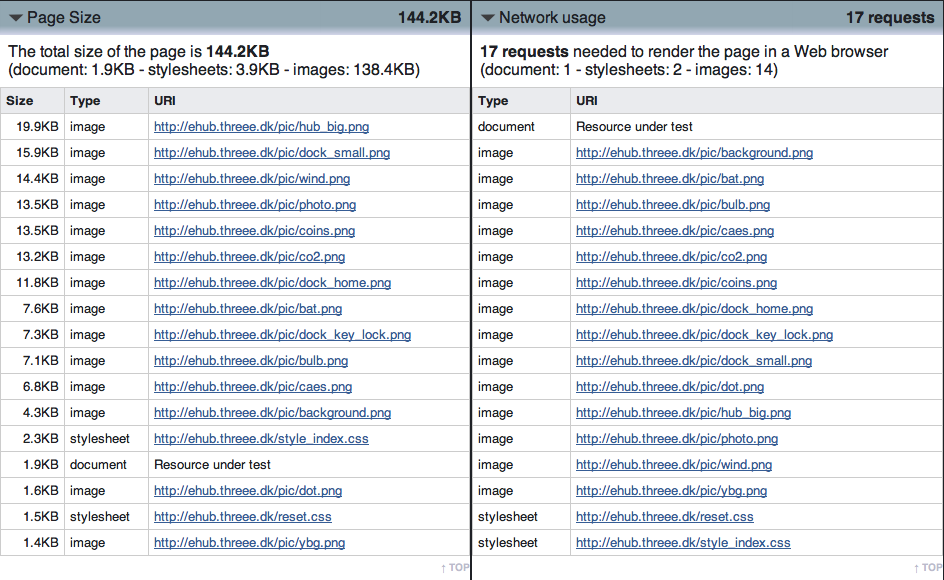
\includegraphics[width=0.8\textwidth]{images/mobileOk2.png}}
   	\caption{Before re-design.}
\end{figure}


\begin{figure}[h!]
	\center
		\setlength\fboxsep{0pt}
		\setlength\fboxrule{1pt}
		\fbox{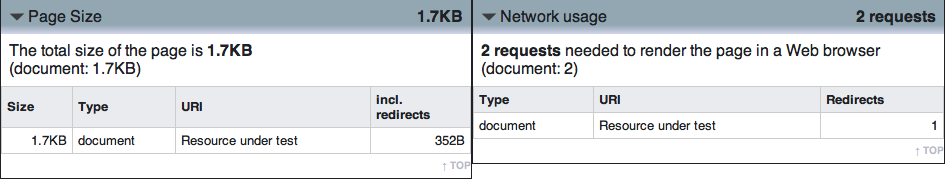
\includegraphics[width=0.8\textwidth]{images/mobileOk1.png}}
   	\caption{After re-design.}
\end{figure}

\section{CSS}  % CSS

CSS is able to get information about almost all newer smartphone devices, information such as orientation and screen size is some information that is retrieved by the browser.

\subsection{Media Queries}

\begin{lstlisting}
	<link rel="stylesheet" type="text/css" media="only screen and (orientation:portrait)" href="portrait.css" />
	<link rel="stylesheet" type="text/css" media="only screen and (orientation:landscape)" href="landscape.css" />
\end{lstlisting}

This line of HTML links to the right CSS document corresponding to the device orientation, in this case CSS3 is used since all devices newer smart phones and tablets support it.

In CSS media queries are conditions that defines if blocks of CSS properties are going to be loaded or not. This will be a great help to re-design a website layout since different pages can be already set to link to this style sheet document. \\
\begin{table}[!h]
	\begin{tabular}{| c | c | p{10.5cm} |}
	\hline
	\textbf{Device} & \textbf{Orientation} & \textbf{Media Queries} \\ \hline
	iPhone & Portrait & @media only screen and (max-width:320px)\\ \hline
	iPhone & Landscape & @media only screen and (max-width:480px)\\ \hline
	HTC, Samsung Galaxy & Portrait & @media screen and (min-width:321px) and (max-width:480px)\\ \hline
	HTC, Samsung Galaxy & Landscape & @media only screen and (min-width:481px) and (max-width:800px)\\ \hline
	iPad, Galaxy & Portrait & @media only screen and (min-width:600px) and (max-width:800px) and (orientation:portrait)\\ \hline
	\end{tabular}
	\caption{Media queries required for the most used tablet computers and smartphones.}
\end{table}

CSS is used to arrange the HTML elements, this documents defines the layout of the page, the use o media queries helps the developer to change only the elements that have a different layout design for the different devices.

The CSS rules has two main parts, the selector and one or more proprieties, the selector is the HTML element, classname or both, the proprieties are style attributes to the element followed by a value for that propriety.

\begin{lstlisting}
	body { width:100%; height: 100%; margin: 0px auto; font-family:Verdana, Geneva, sans-serif; }
\end{lstlisting}

Selector body points to the tag name body on the HTML, being width, height, margin... proprieties at which a value is given.
CSS document is commented for better explanation on the overall layout. 

The module re-design web page follows the same criteria, just the layout is changed with different proprieties.

\section{Validation}
All HTML, CSS and mobile standards are kept and is a valid mobile web page.

\begin{figure}[h!]
		\setlength\fboxsep{0pt}
		\setlength\fboxrule{1pt}
		\fbox{
\includegraphics[width=0.15\textwidth]{images/mobileOk.png}}
\end{figure}
\begin{figure}[h!]
		\setlength\fboxsep{0pt}
		\setlength\fboxrule{1pt}
		\fbox{
\includegraphics[width=0.15\textwidth]{images/vcss.png}}
\end{figure}